
%(BEGIN_QUESTION)
% Copyright 2006, Tony R. Kuphaldt, released under the Creative Commons Attribution License (v 1.0)
% This means you may do almost anything with this work of mine, so long as you give me proper credit

Complete the calibration table for this flow-measuring loop, consisting of an orifice plate, $\Delta$P transmitter, square root extractor, and indicator.  Assume the following instrument ranges:

$$\includegraphics[width=15.5cm]{i00693x01.eps}$$

\begin{itemize}
\item{} FE: 0-400 GPM, 0-125 "W.C. $\Delta$P
\item{} FT: 0-125 "W.C. in, 3-15 PSI out (linear)
\item{} FY: 3-15 PSI in and out (square-root)
\item{} FI: 3-15 PSI in, 0-400 GPM indication
\end{itemize}

% No blank lines allowed between lines of an \halign structure!
% I use comments (%) instead, so that TeX doesn't choke.

$$\vbox{\offinterlineskip
\halign{\strut
\vrule \quad\hfil # \ \hfil & 
\vrule \quad\hfil # \ \hfil & 
\vrule \quad\hfil # \ \hfil & 
\vrule \quad\hfil # \ \hfil & 
\vrule \quad\hfil # \ \hfil & 
\vrule \quad\hfil # \ \hfil \vrule \cr
\noalign{\hrule}
%
% First row
Flow rate & Percent of & Orifice $\Delta$P & FT output & FY output & FI indication \cr
%
% Another row
(GPM) & max. flow (\%) & ("W.C.) & signal (PSI) & signal (PSI) & (GPM) \cr
%
\noalign{\hrule}
%
% Another row
 & 0 &   &   &   &  \cr
%
\noalign{\hrule}
%
% Another row
  & 10 &   &   &   &  \cr
%
\noalign{\hrule}
%
% Another row
  & 25 &   &   &   &  \cr
%
\noalign{\hrule}
%
% Another row
 & 50 &   &   &   &  \cr
%
\noalign{\hrule}
%
% Another row
  & 75 &   &   &   &  \cr
%
\noalign{\hrule}
%
% Another row
  & 90 &   &   &   &  \cr
%
\noalign{\hrule}
%
% Another row
 & 100 &   &   &   &  \cr
%
\noalign{\hrule}
} % End of \halign 
}$$ % End of \vbox

\underbar{file i00693}
%(END_QUESTION)





%(BEGIN_ANSWER)

% No blank lines allowed between lines of an \halign structure!
% I use comments (%) instead, so that TeX doesn't choke.

$$\vbox{\offinterlineskip
\halign{\strut
\vrule \quad\hfil # \ \hfil & 
\vrule \quad\hfil # \ \hfil & 
\vrule \quad\hfil # \ \hfil & 
\vrule \quad\hfil # \ \hfil & 
\vrule \quad\hfil # \ \hfil & 
\vrule \quad\hfil # \ \hfil \vrule \cr
\noalign{\hrule}
%
% First row
Flow rate & Percent of & Orifice $\Delta$P & FT output & FY output & FI indication \cr
%
% Another row
(GPM) & max. flow (\%) & ("W.C.) & signal (PSI) & signal (PSI) & (GPM) \cr
%
\noalign{\hrule}
%
% Another row
0 & 0 & 0 & 3 & 3 & 0 \cr
%
\noalign{\hrule}
%
% Another row
40 & 10 & 1.25 & 3.12 & 4.2 & 40 \cr
%
\noalign{\hrule}
%
% Another row
100 & 25 & 7.81 & 3.75 & 6 & 100 \cr
%
\noalign{\hrule}
%
% Another row
200 & 50 & 31.25 & 6 & 9 & 200 \cr
%
\noalign{\hrule}
%
% Another row
300 & 75 & 70.31 & 9.75 & 12 & 300 \cr
%
\noalign{\hrule}
%
% Another row
360 & 90 & 101.25 & 12.72 & 13.8 & 360 \cr
%
\noalign{\hrule}
%
% Another row
400 & 100 & 125 & 15 & 15 & 400 \cr
%
\noalign{\hrule}
} % End of \halign 
}$$ % End of \vbox


%(END_ANSWER)





%(BEGIN_NOTES)

%INDEX% Calibration: table, flow transmitter
%INDEX% Measurement, flow: calibration table

%(END_NOTES)


